\documentclass[12pt]{article}
\usepackage{url}
\usepackage[margin=1.1in]{geometry}
\usepackage{graphicx}
\usepackage{float}
\usepackage{listings}
\usepackage[hidelinks]{hyperref}

\title{Companion Cube Calculator \\ User Guide}
\author{Geneva Smith (GenevaS)}
\date{\today}

\begin{document}
\maketitle

\textit{The repository for this project can be found at 
\href{https://github.com/GenevaS/CAS741}{https://github.com/GenevaS/CAS741}.}
\\

The Companion Cube Calculator ($C^3$) is a mathematical tool for determining 
the range of a user-specified function given the domains of the function's 
variables. The calculations are performed using interval arithmetic and only 
closed, real intervals ($[a,b]$) are supported.

The tool is restricted to the following operators:
\begin{itemize}
	\item Addition ($+$)
	\item Subtraction ($-$)
	\item Multiplication ($*$) 
	\item Division ($/$) \\ \textbf{Note}: You cannot specify a divisor 
	interval that contains zero ($0$).
	\item Exponentiation (\^{})  \\ \textbf{Note}:	
	\begin{itemize}
		\item Base numbers ($B^x$) must be greater than $1$.
		\item Exponents ($x^N$) must be greater than or equal to zero (0), and 
		must be a whole number.
		\item You cannot specify both the base number and the exponent as 
		intervals.
	\end{itemize}
\end{itemize} 

Implicit multiplication, constant values, and round brackets (``()") are 
supported by the $C^3$ tool.

\textbf{Note}: If you copy values from PDFs into the $C^3$ tool, your data 
might not be processed correctly.

Full documentation for the software can be found at:
\begin{center}
	\url{https://github.com/GenevaS/CAS741/tree/master/Doc}
\end{center}

\paragraph{System Requirements\\}
The $C^3$ tool can only be run on Windows operating systems.

\paragraph{Using the $C^3$ Tool\\}
The $C^3$ tool (Figure~\ref{fig_gui}) has two work flows for accepting your 
inputs -- direct input and loading from a file. 

\begin{figure}[th]
	\centering
	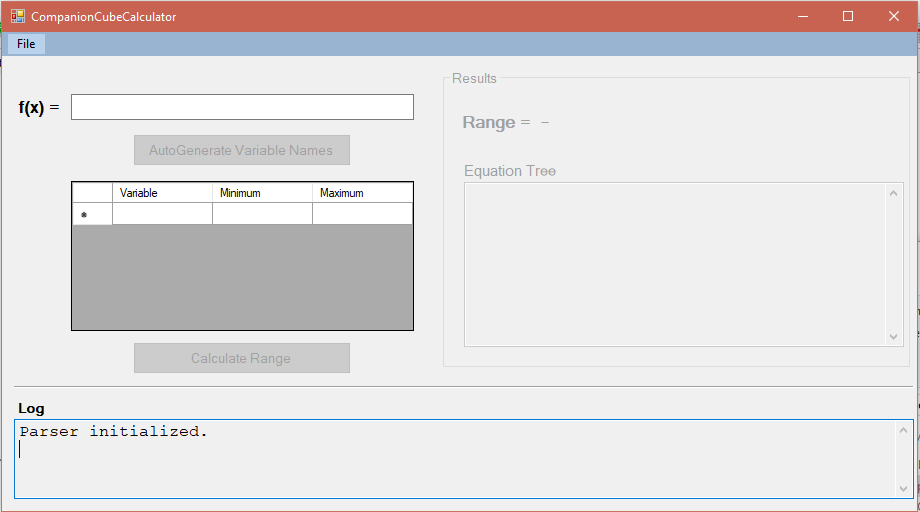
\includegraphics[width=\textwidth]{figures/C3GUI}
	\caption{The $C^3$ tool}
	\label{fig_gui}
\end{figure}

\subparagraph{Direct Input\\}
In the direct input work flow, you enter your equation and variable domains 
into the $f(x)$ text box and variable table respectively. The range of your 
equation is calculated by clicking the ``Calculate Range" button. This button 
will not be enabled until the tool detects values in the $f(x)$ field and each 
named row in the variable domain table.

To make this work flow simpler, the tool contains an ``AutoGenerate Variable 
Names" button which becomes enabled when you enter your equation into the 
$f(x)$ field. This button automatically populates the ``Variable" column 
of the domain table 
with the variables found in your equation. You must manually enter in the 
values for the minimum and maximum bounds.

\subparagraph{Loading from a File\\}
You can load function and variable domain data into the tool 
from a file using the File $\rightarrow$ Load menu option. The tool will 
automatically calculate the results.

Only text files (*.txt) are supported at this time. You must only put one value 
per line in your input file. The expected format of the file is:

\begin{itemize}
	\item The first line of the file contains your function.
	\item Each subsequent line contains the information for one of your 
	variable domains, where each field is separated by a comma (,).
\end{itemize}

\textbf{Example}:

Given the equation $f(x) = x + y, x = [2, 4], y = [3, 5]$, the corresponding 
file 
would contain:

 \begin{lstlisting}
 f(x) = x + y
 x,2,4
 y,3,5
 \end{lstlisting}
 
 You can optionally omit the equality in your user function:
 
\begin{lstlisting}
x + y
x,2,4
y,3,5
\end{lstlisting}

You can find the sample file, \texttt{test.txt}, corresponding to this example 
\texttt{TestFiles} directory.

\paragraph{Reading the Results\\}
You can find the calculated range of your function in the ``Range" field. You 
cannot edit this field at any time.

The ``Equation Tree" field contains the calculation tree followed during 
processing. If you are not getting the results that you expect, this 
information might help you identify how operator precedence is affecting how 
values are used. You can edit this field when it contains information, but no 
changes will be saved.

\end{document}